% !TEX encoding = UTF-8 Unicode
% This is based on the LLNCS.DEM the demonstration file of
% the LaTeX macro package from Springer-Verlag
% for Lecture Notes in Computer Science,
% version 2.4 for LaTeX2e as of 16. April 2010
%
% See http://www.springer.com/computer/lncs/lncs+authors?SGWID=0-40209-0-0-0
% for the full guidelines.
%

\documentclass{llncs}
\usepackage[utf8]{inputenc}
\usepackage{graphicx}


\begin{document}

\title{Optimización a Gran Escala usando Algoritmos Genéticos: Mutación Selectiva Adaptativa}
%
\titlerunning{Optimización a gran Escala}  % abbreviated title (for running head)
%                                     also used for the TOC unless
%                                     \toctitle is used
%
\author{Juan Pablo Salamanca Ramírez}
%
\authorrunning{Juan P. Salamanca} % abbreviated author list (for running head)
%
%%%% list of authors for the TOC (use if author list has to be modified)
\tocauthor{}
%
\institute{Departamento de Ingenieria de Sistemas e Industrial, Universidad Nacional de Colombia, Bogotá, Carrera 45 No 26-85, Colombia,\\
\email{jpsalamarcara@unal.edu.co}}

\maketitle

\begin{abstract}
...
\keywords{evolutionary computation, evolutionary algorithm, real optimization, large scale}
\end{abstract}
%



\section{Introducción}
Los problemas de optimización están presentes en la vida diaria de todos los seres humanos, el hecho de preguntarse ¿Cómo hacer un bueno uso del dinero disponible? cuando vas de compras al supermercado o ¿Cuál es la mejor forma de llegar a la escuela? haciendo uso de los diferentes medios de transporte de una ciudad, es plantearse un problema de optimización. Aunque existen diversas técnicas de optimización, una de las más apreciadas en la comunidad académica y en la industria, son los algoritmos genéticos. En este documento se presenta una propuesta de algoritmo genético para optimización de funciones en el dominio de los números reales, haciendo frente al problema de la no separabilidad.

%Fin de la Introducción
\section{Estado del Arte}
En la actualidad existen diversas técnicas de optimización para el dominio de los números reales. Algunas de estas son muy conocidas, sin embargo, tienen muchas condiciones particulares para poderse usar correctamente. Por ejemplo, para aplicar el gradiente descendente, la función a optimizar debe ser diferenciable y el manejo de las restricciones puede volverse todo un dolor de cabeza. Otras técnicas no dependientes de gradientes o derivadas. suelen tener  resultados muy buenos, sin embargo, estas sufren la maldición de la dimensionalidad, es decir, cuando las dimensiones del problema crecen, sus soluciones ya dejan de ser tan buenas. En este grupo se encuentran los algoritmos genéticos, los cuales pueden describirse como una búsqueda aleatoria bio inspirada en la teoría de la evolución.
Muchos investigadores han intentado resolver problemas de optimización sobre el dominio de los reales, aplicando diferentes variantes de algoritmos genéticos. Por ejemplo, el algoritmo HaEA \cite{gomez} hace que la selección de sus operadores de cruce y mutación sea aleatoria y auto adaptable, lo cual lo libera de muchos parámetros y hace que sea muy eficiente. Otras técnicas pertenecientes a la computación evolutiva, hacen frente a la optimización con estrategias distintas. Como es el caso de la optimización multi-objetivo, la cual toma base en el concepto de dominancia entre individuos de una población y dividiendo el problema general en pequeños problemas manejables \cite{zitzler:laumans:thiele}. Sin embargo, el inconveniente de muchas de estas técnicas, radica en la naturaleza de la función a optimizar. En muchos casos, las funciones son separables, es decir, sus variables de entrada no presentan interdependencia, en este caso, podríamos dividir el conjunto de variables de entrada y hacer optimización multi-objetivo. O hacer una búsqueda aleatoria optimizando una a una las variables de entrada. Sin embargo, las funciones reales, no suelen tener este tipo de naturaleza aprovechable \cite{caaman}. 
En los últimos años han surgido novedosas técnicas de acuerdo a la separabilidad o no separabilidad de una función a optimizar. Esto crea la molesta tarea de estudiar analíticamente la función objetivo para identificar su naturaleza.

\section{Propuesta}
Teniendo en cuenta las principales conclusiones de J. Gómez \cite{gomez} en relación a la preservación de la diversidad como estrategia evolutiva y al análisis de los diferentes esquemas de selección realizado por T. Blicke \& L. Thiele\cite{blick:thiele}; se plantea encontrar un método para seleccionar individuos de una población, en el cual se favorezca la   exploración y explotación como principios básicos para disminuir la perdida de diversidad y la probabilidad de estancamiento en un máximo (o mínimo) local. El resultado es un híbrido entre la selección por ruleta y la selección por ranking.

\subsection{Estrategia de Selección: Ruleta-Ranking}
El procedimiento de selección propuesto, llamado inicialmente Ruleta-Ranking, se describe paso a paso a continuación:
\begin{enumerate}
\item Se normalizan las medidas de aptitud de cada individuo de la población usando escala decimal.
\item Se normalizan los datos del paso anterior en el intervalo $[0,1]$
\item Se ordenan de forma descendente los individuos de acuerdo su medida de aptitud normalizada, de manera que el mejor individuo sea el primero de la lista y el peor el último.
\item Generar un número aleatorio usando una distribución normal con $\mu=0$ y $\sigma=\frac{1}{3}$, y aplicarle la función valor absoluto.
\item Seleccionar el individuo con la medida de aptitud normalizada inmediatamente mayor al número aleatorio generado en el paso anterior.
\item Retirar al individuo seleccionado de la lista y ajustar las probabilidades de los individuos restantes.
\end{enumerate}
En esta estrategia, los mejores individuos tienen mayor probabilidad de ser seleccionados inicialmente, sin embargo, con su salida de la lista de espera, se redistribuye la probabilidad en los individuos restantes, ofreciéndole prioridad a los nuevos mejores. Esta técnica permite exploración ya que por la forma de la distribución normal, existe la probabilidad de seleccionar individuos no tan buenos. Y permite explotación, porque se seleccionan los mejores en mayor proporción. 
Para controlar la complejidad del algoritmo, se mantiene la sumatoria total de las medidas de aptitud normalizadas de los individuos en espera y cada vez que alguno es elegido, su medida de aptitud es restada del total y se aplica otra normalización respecto a este nuevo total solamente cuando se lanza nuevamente la ruleta.

\paragraph{Comentario.}
Al cambiar la forma de la distribución del número generado en el paso $4$, por una con $\mu=1$, se obtiene que la ejecución del algoritmo genético minimiza la función de aptitud.

\subsection{Estrategia de Generación y Reemplazo}
Para la generación de nuevos individuos se propone como estrategia el matrimonio, generando de a dos hijos por pareja. Sin embargo, el criterio de selección de pareja se dividió en dos: por similitud y por mejor medida de aptitud, teniendo en cuenta que el mejor individuo tiene $n-1$ oportunidades de elegir, el segundo mejor individuo tiene $n-2$ y así sucesivamente hasta que el penúltimo individuo solo pudiese elegir al peor ($n$ es el tamaño total de los individuos elegibles).

Como estrategia de reemplazo se propuso el estado estable y reemplazo generaciónal, en combinación con alguna de las estrategias de generación anteriormente descritas.

\subsection{Función de Aptitud}
La función de aptitud es una función de las quince funciones disponibles en \cite{IEEE:CEC} , la cuales fueron usadas para la competencia de optimización a gran escala organizada por la IEEE en 2013. 
Estas funciones cuentan con 1000 variables de entrada y presentan diversas carecteríscas de separabilidad.
\subsection{Inicialización}
Para la inicialización se generan cadenas de números aleatorios, bajo una distribución normal con $\sigma=1$ y $\mu=0$ 

\subsection{Operadores}
En cuanto a los operadores se tienen dos, mutación y cruce. 
\subsubsection{Mutación}
Para la mutación, se propone un operador auto adaptable y selectivo. Para lograr esto, se define un radio de búsqueda con centro en el valor de la $i-$ésima variable de cada individuo, este radió esta definido por una distribución normal con $\sigma=$ tasa de aprendizaje del individuo, valor que a su vez, fue asignado inicialmente siguiendo otra distribución de probabilidad normal. Esta tasa de aprendizaje, será ajustada de acuerdo a la regla de $\frac{1}{5}$. Sin embargo, todavía queda la incógnita de como hacer frente a la no separabilidad. 
Tomando inspiración en la auto adaptabilidad de HaEA  \cite{gomez} para seleccionar sus operadores, se propuso detectar la sensibilidad de cada una de las variables de la función objetivo al ser modificadas, teniendo en cuenta, que posiblemente durante todo el proceso de optimización esta sensibilidad podría disminuir o aumentar de acuerdo al estado de las demás variables. La solución fue premiar o castigar las variables que después de aplicarles una mutación aumenten o disminuyan la medida de aptitud del individuo. Sin embargo, si por cada variable mutada se midiera el cambio en la medida de aptitud, aumentaría la complejidad del algoritmo, entonces, la solución fue usar el mecanismo ya conocido para premiar o castigar la tasa de aprendizaje usando la regla de $\frac{1}{5}$, para adicionalmente premiar la sensibilidad de cada variable mutada y no abusar de la función de aptitud.
Cabe aclarar, que de acuerdo a la sensibilidad de cada variable, aumenta o disminuye la probabilidad de mutar esa variable.
Por otra parte, queda la posibilidad de que una o más variables sean lo suficientemente castigadas como para que la población se quede en un mínimo (o máximo) local. Para hacer frente a este problema se propuso el mecanismo de insertar ruido en la sensibilidad acumulada de las variables. Para que nuevamente se empiece a adaptar dicha sensibilidad y sea cambiante en el transcurso de la optimización. Este proceso es aleatorio y está definido por una probabilidad $p$ como parámetro de entrada.

\subsubsection{Cruce}
El operador de cruce es sumamente sencillo, se selecciona un punto pivote en la cadena de variables de cada individuo y a partir de este son generados dos nuevos individuos, a los cuales se les asigna la tasa de aprendizaje y la sensibilidad de alguno de sus dos progenitores.

\section{Experimentos y Resultados}
Para determinar cual de las estrategias evolutivas es mejor para complementar esta propuesta, se corrieron varias pruebas: 
Para una estrategia reemplazo de estado estable, se encontraron mejores soluciones para las funciones ${F5,F6,F9,F10}$ a diferencia de las demás que era optimizadas muy rápidamente por una estrategia de reemplazo generacional. 
En cuanto a la estrategia de generación de nuevos individuos, los matrimonios realizados por similitud demostraron ser más lentos que los matrimonios por mejor medida de aptitud.

\subsection{Ejecución}
Se ejecutó la implementación usando las cuatro posibles combinaciones de estrategias evolutivas propuestas, sobre la función $F1$:
Reemplazo generacional con matrimonio por mejor medida de aptitud \ref{Ejecucion_1}, reemplazo generacional con matrimonio por similitud \ref{Ejecucion_3}, reemplazo de estado estable con matrimonio por mejor medida de aptitud \ref{Ejecucion_2} y reemplazo de estado estable con matrimonio por similitud \ref{Ejecucion_4}. Fijando como parámetros el tamaño de la población en 100, 10000 en el total de iteraciones y el parámetro $p=0.01$.

\begin{figure}
  \centering
    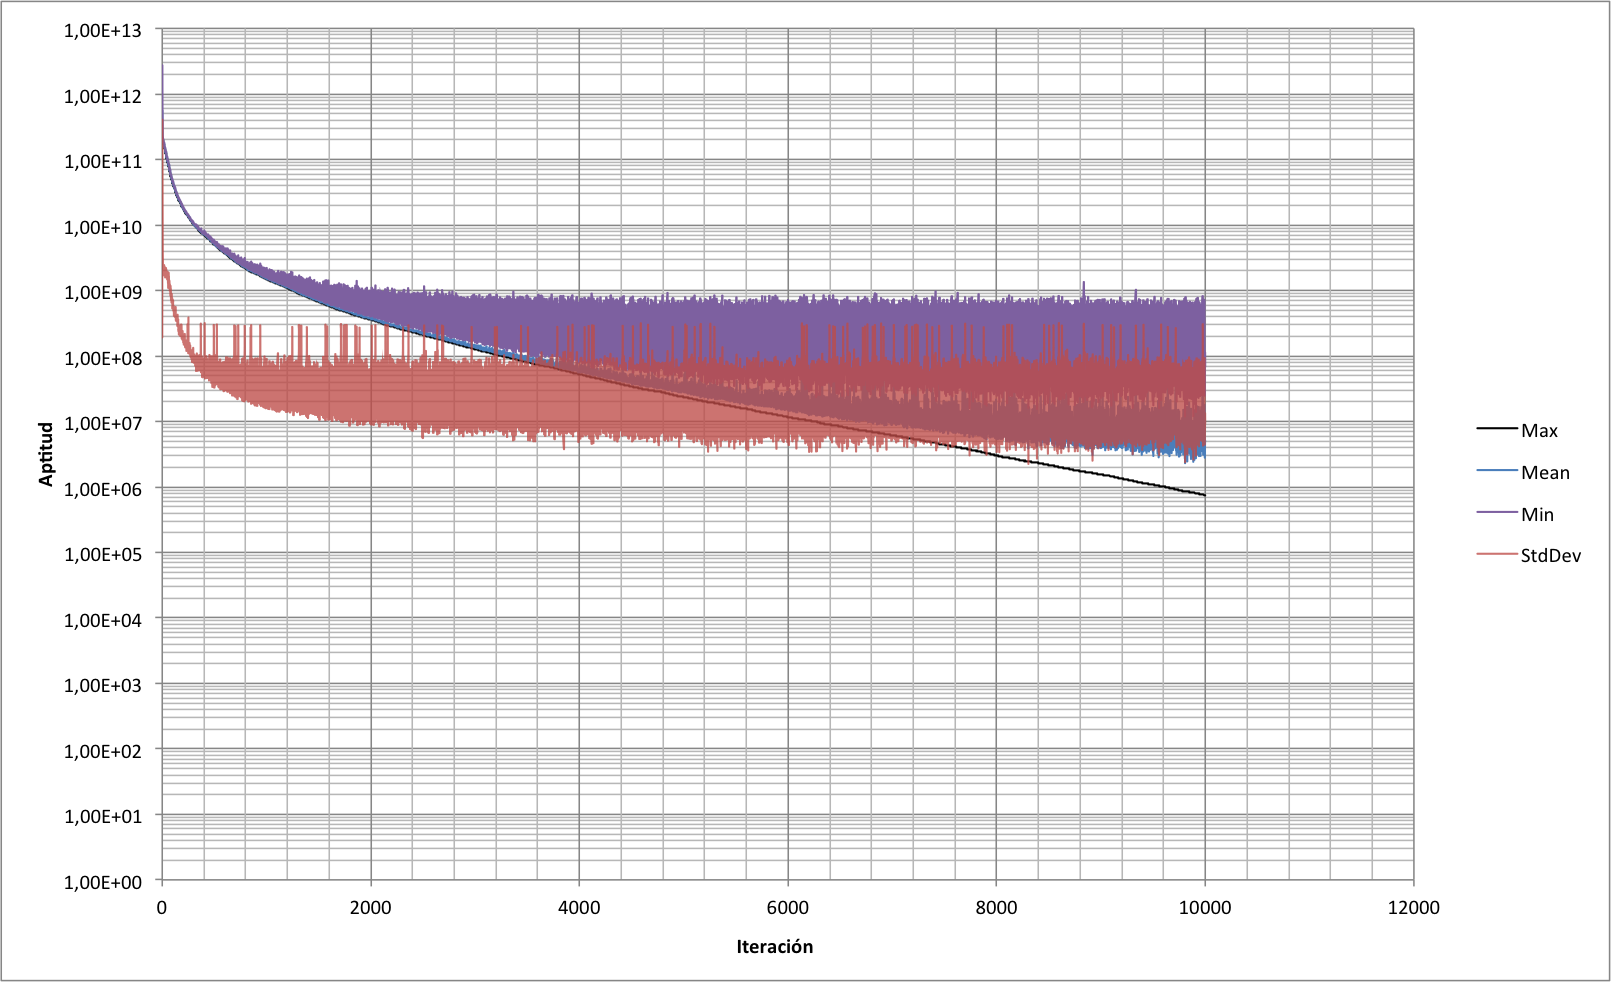
\includegraphics[width=0.95\textwidth]{bestFitGen}
  \caption{Matrimonio por Mejor Aptitud  y Reemplazo Generacional en $F1$}
  \label{Ejecucion_1}
\end{figure}


\begin{figure}
  \centering
    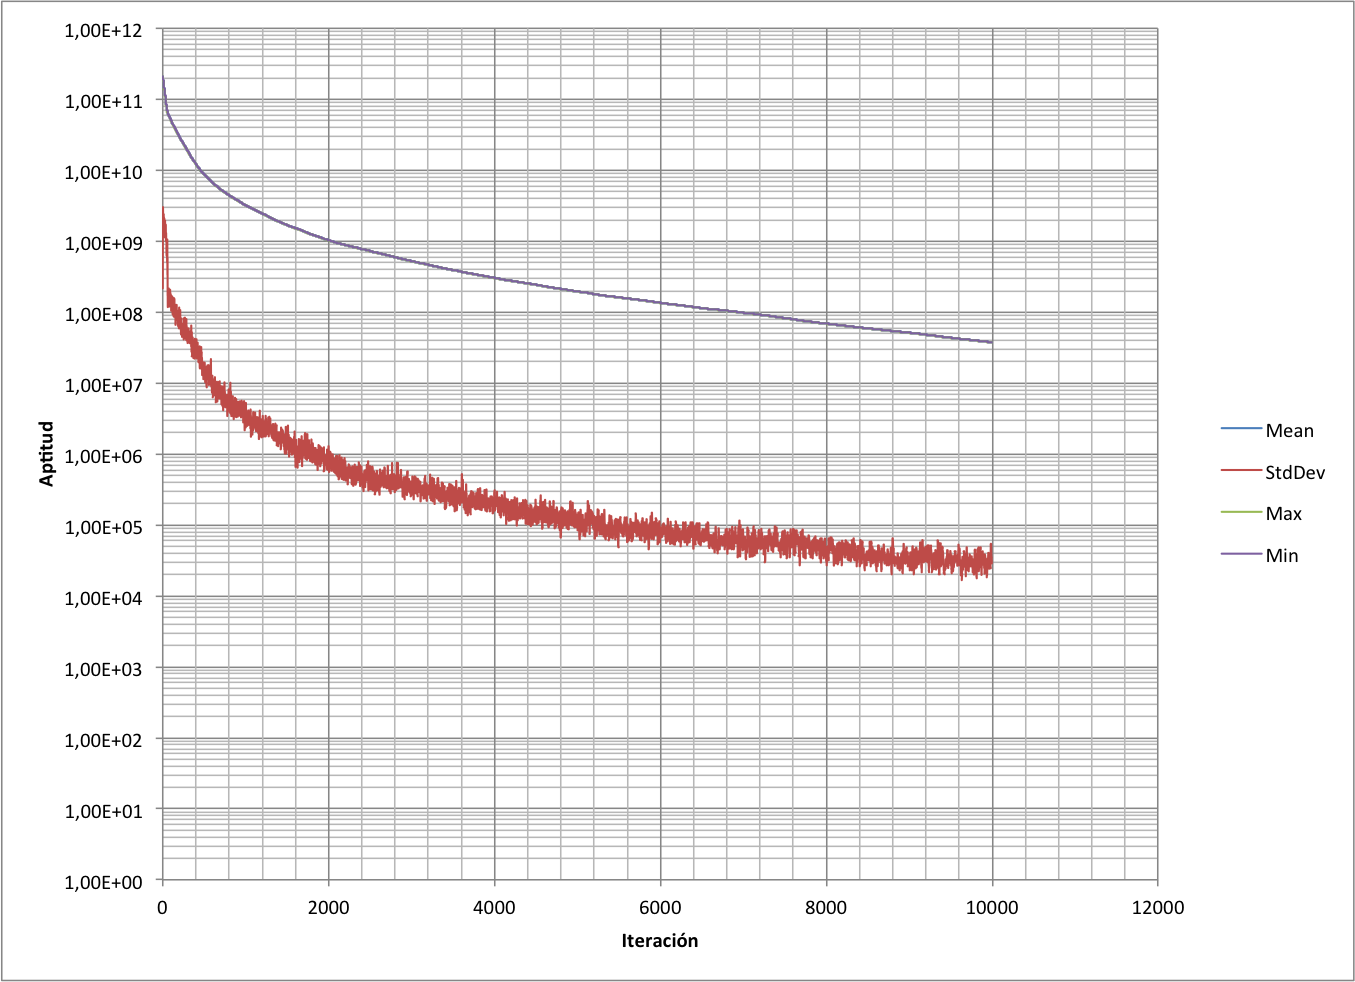
\includegraphics[width=0.95\textwidth]{bestFitSteady}
  \caption{Matrimonio Mejor Aptitud  y Reemplazo de Estado Estable en  $F1$}
  \label{Ejecucion_2}
\end{figure}


\begin{figure}
  \centering
    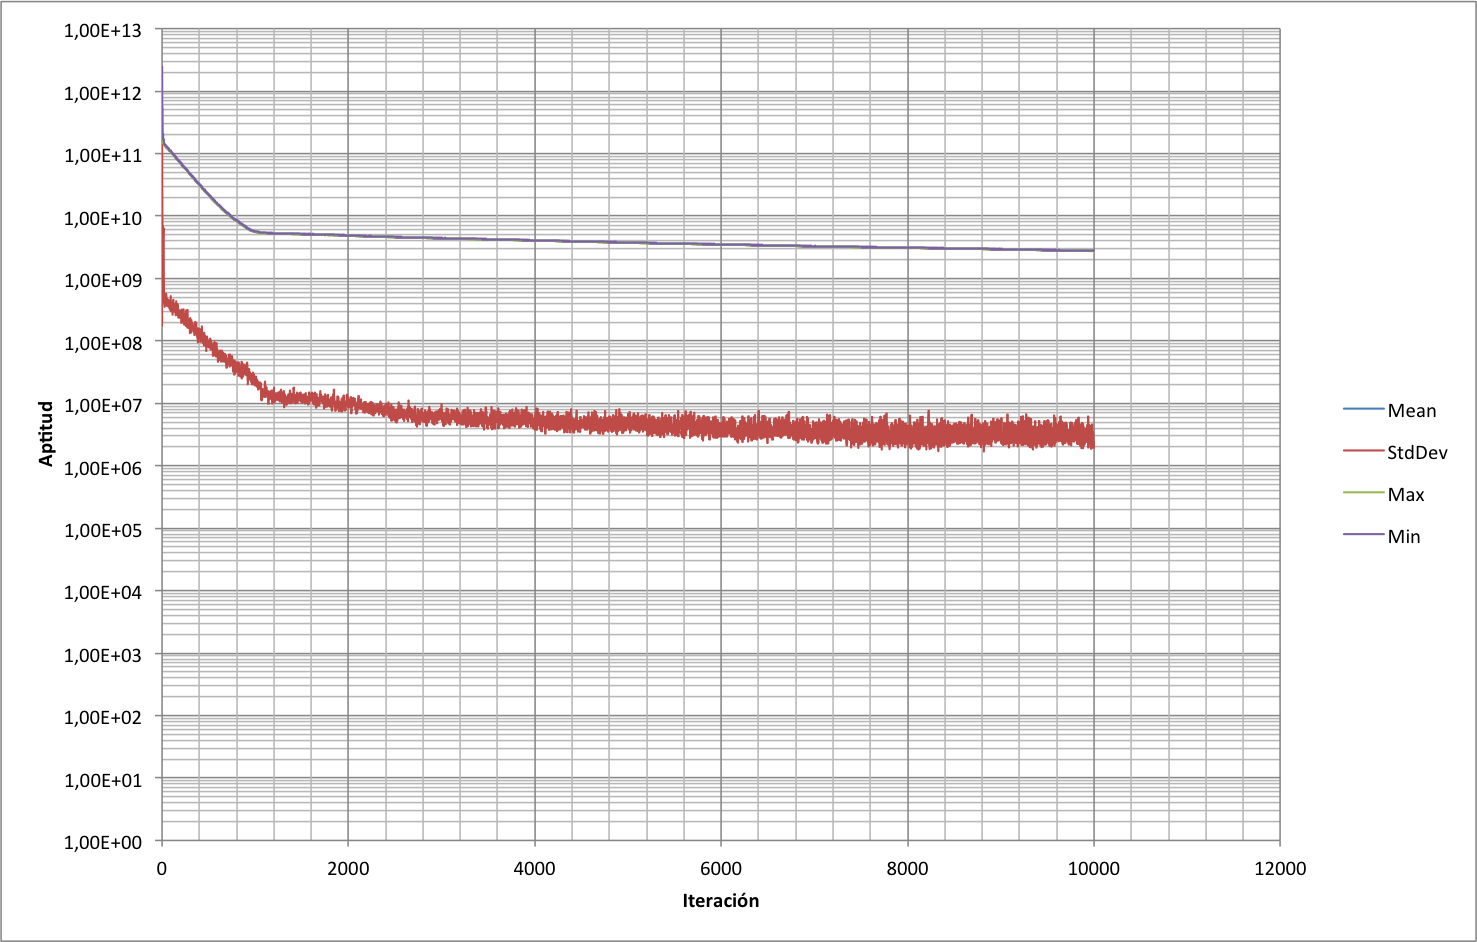
\includegraphics[width=0.95\textwidth]{similarityGen}
  \caption{Matrimonio por Similitud  y Reemplazo Generacional en $F1$}
  \label{Ejecucion_3}
\end{figure}

\begin{figure}
  \centering
    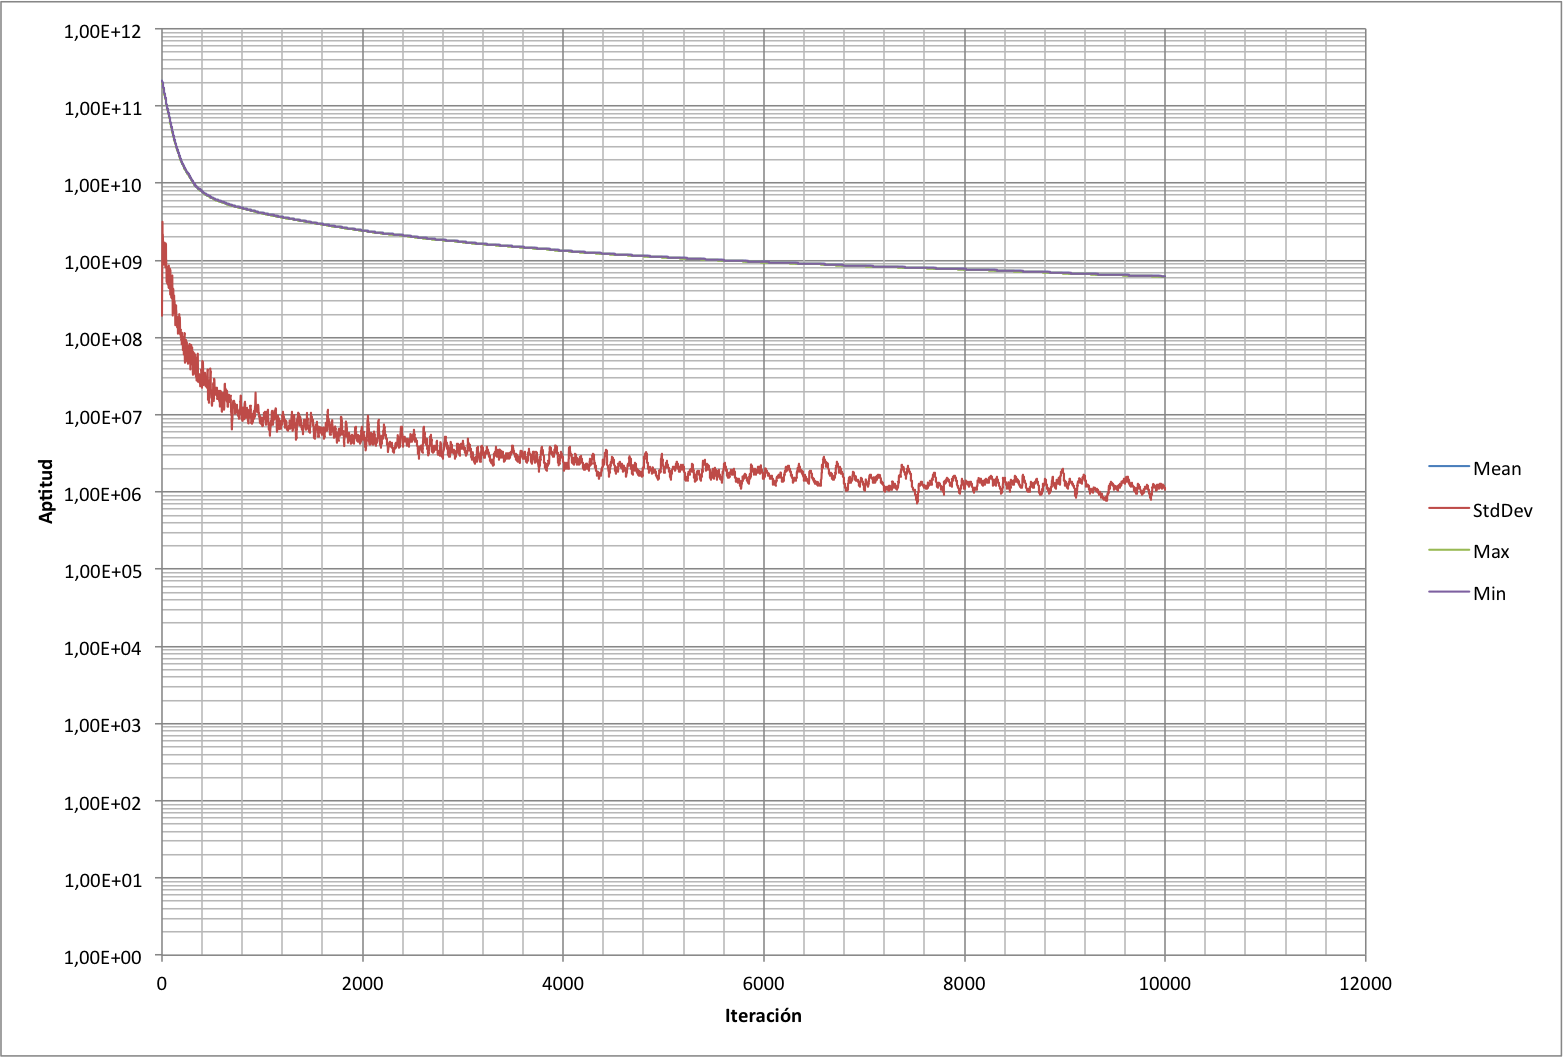
\includegraphics[width=0.95\textwidth]{similaritySteady}
  \caption{Matrimonio por Similitud  y Reemplazo de Estado Estable en $F1$}
  \label{Ejecucion_4}
\end{figure}

\section{Conclusiones}

\begin{itemize}
\item ...
\end{itemize}

\begin{thebibliography}{5}
%

\bibitem {gomez}
J. Gómez:
Self Adaptation of Operator Rates in Evolutionary Algorithms
Universidad Nacional de Colombia and The University of Memphis, (2004)

\bibitem {IEEE:CEC}
X. Li, K. Tang, M. Omidvar, Z. Yang and K. Qin, "Benchmark Functions for the CEC'2013 Special Session and Competition on Large Scale Global Optimization," Technical Report, Evolutionary Computation and Machine Learning Group, RMIT University, Australia, 2013.

\bibitem {blick:thiele}
Tobias Blickle \& Lothar Thiele:
A Comparison of Selection Schemes used in Genetic Algorithms.
Computer Engineering and Communication Networks Lab.
Swiss Federal Institute of Technology. (1995)

\bibitem {zitzler:laumans:thiele}
Eckart Zitzler, Marco Laumanns, and Lothar Thiele,
SPEA2: Improving the Strength Pareto Evolutionary Algorithm
Computer Engineering and Networks Laboratory (TIK),
Department of Electrical Engineering,
Swiss Federal Institute of Technology (ETH) Zurich (2001)

\bibitem{caaman}
Pilar Caamaño*, Francisco Bellas, Jose A. Becerra, Richard J. Duro, Evolutionary algorithm characterization in real parameter optimization problems, Applied Soft Computing 13 (2013) 1902–1921

\end{thebibliography}

\end{document}

